\section{Design process and verifications}
	With the data obtained from the preliminary analysis, the design has been carried using the 3D CAD software \texttt{AutoDesk Inventor Professional} with the help of the components library provided by the manufacturer Parker IPS. At this stage what we mainly did was to \textit{give shape} at the chosen concept by using mechanical elements provided by the library only in order to minimize the need of custom-made parts.
	
	For actuating the machine no off-the-shelf solution are available, hence we decided to create our custom rack design (\textbf{INSERIRE E CREARE RIFERIMENTO AL DISEGNO}): such component is made by a set of smaller bid that can be 3D printed with plastic material; such elements can be joined together by means of standard T-slot components. The rack is mounted on both tracks placed at the ground (motion in the $x$ direction) and the elevated one (motion in the $y$ direction); the gear attached to the motor that's actuating the system is a standard element made out of steel. Proper static verification of the component will be described in the following pages.
	
	Using the theory from the course we performed a static verification of the machine and we verified two critical bolted joints.
	
	\subsection{Static verification}
	With all the geometrical values known, it has been possible to carry out a more detailed analysis. Considering a more complex model of the forces that takes into account also the distributed load due to the gravity and that the force $F$ is applied with an eccentricity $e=5cm$, it has been possible to parametrically define the hyperstatic variables as
	\[ X_1 \simeq \big( 0.63-0.16\zeta\big) N\cdot m \qquad X_2 \simeq -8.10 \ N\cdot m \] \[ X_3 \simeq \big( - 10.54 - 11.07\zeta + 55.53\zeta^2 - 6.17\zeta^3 \big) N\cdot m \]
	Evaluating the stress state on the 3 beams making up the structure for values of $\zeta \in [0,L]$, what we obtained is that the most critical section is in the elevated track for $\zeta^* = 1.65m$ at $z^* = 1.65m$ where the maximum bending value $M_x^* \simeq 135.64N\cdot m$ is achieved. Knowing that $N^* = 0$ and neglecting the shear stress contribution due to both shear $V_y^* \simeq 111N$ and torque $M_z^* \simeq 1.89N\cdot m$, the stress state is
	\[ \sigma_{zz}(y) = \frac{M_x^*}{I_{xx,track}}y \qquad \Rightarrow \qquad \sigma_{zz,max} = \sigma_{zz}(2cm) \simeq 28.68 MPa   \]
	This leads to a safety factor of $\phi = \sigma_{ys}/\sigma_{zz,max} \simeq 8.37$, meaning that the structure is statically verified. This value is more then twice than the one achieved in the preliminary design phase but is due to the fact that in this case the full analytical solution of the hyperstatic problem has been considered, having determined all geometrical properties of the sections. As a reminder:
	\begin{itemize}
		\item due to the lack of analytical formulas for such complex geometry section, shear components due to torque and shears are neglected and could have influenced the mechanical system;
		\item we did not consider external forces acting that might act on the global $x$ axis due to the actuation of the machine or accidental load applied by the end user: this can lead to an increase in bending and torques that might make the system fail.
	\end{itemize}

	\textbf{MAGARI AGGIUNGERE GRAFICI DEL MOMENTO IN FUNZIONE DI 2/3 VALORI DI $\zeta$}
	
	\textbf{AGGIUNGERE LA STIFFNESS VERIFICATION}
	\subsection{Fatigue verification}
	\paragraph{Most critical section} As already stated, the most critical section is subjected to a maximum stress of $\sigma_{max} \simeq 28.68MPa$. While functioning we expect that the turret performing the operation to the soil periodically moves along the track: having $\zeta$ varying over time determines that also the internal loads are fluctuating and this might arise fatigue failure of the machine.
	
	Given the need of a fatigue verification, acknowledged that the minimum bending load at $z^*$ is $M_{x,min} \simeq 14.05N\cdot m$ achieved for $\zeta = 0m$, determining $\sigma_{min} \simeq 2.97MPa$; this further implies that the mean and amplitude stresses for fatigue verification are
	\[ \sigma_m \simeq 15.82 MPa \qquad \sigma_a \simeq 12.85MPa \]
	According to Soderberg criterion, the equivalent amplitude only stress component evaluates to
	\[ \sigma_{a,eq} = \frac{\sigma_{ys} \sigma_a}{\sigma_{ys} - \sigma_m} \simeq 13.76MPa  \] 
	In this case the load factor is $C_l=1$; given an equivalent diameter $d_{eq} = \sqrt{\frac 4\pi A} = 29mm$, the corresponding size factor is $C_d = 1.189d_{eq}^{-0.097} \simeq 0.86$; details concerning the surface finish of the T-slot beams are not enough to fully determine the surface coefficient $C_s$ that's assumed in this case to be $0.8$ as safety value. Considering an endurance limit of the 6061-T5 aluminium alloy of $\sigma_{lim} = 100MPa$ \cite{aluminium-endurance}, this means that the safety factor against fatigue failure is
	\[ \phi_\textrm{fatigue} = C_sC_dC_l\frac{\sigma_{lim}}{\sigma_{a,eq}} \simeq 4.98 \]
	\subsection{Threaded joints verification}
\subsubsection*{Preliminary design}
Given the customer's requirements, the threaded fasteners used for the threaded joints in the whole robot are chosen to be standard screws with diameter of $8mm$, compatible with the $40mm$ T-slot profiles.

Considering the threaded joints present on the robot, the maximum thickness of the members is given by the sum between the beam cross section's width, $40 mm$, and the machined gussets thickness, $8 mm$. Given that two screws must fit, as in section $A$, the length of the screws is chosen to be equal to $18 mm$, according to \texttt{UNI ISO 888}; table \ref{tab:boltchoise} reports main properties of the chosen bolt used for the verification of the connections.

\begin{table}[bt]
	\rule{\linewidth}{2pt}
	\caption{selected bolt chosen from the Parker IPS catalogue \cite{parker-ds} and related main properties.}
	\label{tab:boltchoise}
	\rule{\linewidth}{1pt} 
	\begin{center}
	\begin{tabular}{r c c}
		Parameter & symbol & value \\ \hline
		diameter & $d$ & $8mm$ \\
		head diameter & $d_0$ & $14mm$ \\
		length & $l$ & $18mm$ \\
		cross-section & $A_b$ & $16\pi mm^2$ \\
		tensile cross-section & $A_{bt}$ & $36.6mm^2$ \\
		ultimate tensile strength & $\sigma_{uts}$ & $505MPa$ \\
		product code & \multicolumn{2}{c}{\texttt{24-118-8}}
	\end{tabular}
	\end{center}
	\rule{\linewidth}{2pt}
\end{table}

With reference to Figure \ref{fig:freebodydiagramframe}, threaded joints are present in sections $A$, $B$, $C$ and $D$. The verifications are carried out with respect to the most critical sections which, according to the load analysis performed previously, are identified as section $A$ and $D$. Moreover, since the load distribution depends on the position of the point of application of the external load, the most critical condition corresponds to the one in which the load is applied in $\zeta = 1$ for section $A$ and $\zeta = 3$ for section $D$.\\
%volevo fare subsubsection per le sezioni A e D
\subsubsection*{Section A}
The loads applied on section $A$ are the following:\\
\begin{itemize}
	\item axial load $N_{A} = -251.126 N$;
	\item bending moment $M_{xA} = -12.645 N\cdot m$; 
	\item bending moment $M_{yA} = 1.894 N\cdot m$; 
	\item torque $M_{zA} = -0.594 N\cdot m$.
\end{itemize}
In correspondence of section $A$, there are two machined gussets chosen from the Parker IPS catalogue \cite{parker-ds}, reported in figure \ref{fig:gusset}.
Given the geometry of the component, the threaded joints are positioned on the vertical $z$ and horizontal $x$ global axis.  For this reason, two separated analysis are performed. 
\begin{SCfigure}[1.5][bht]
	\centering
	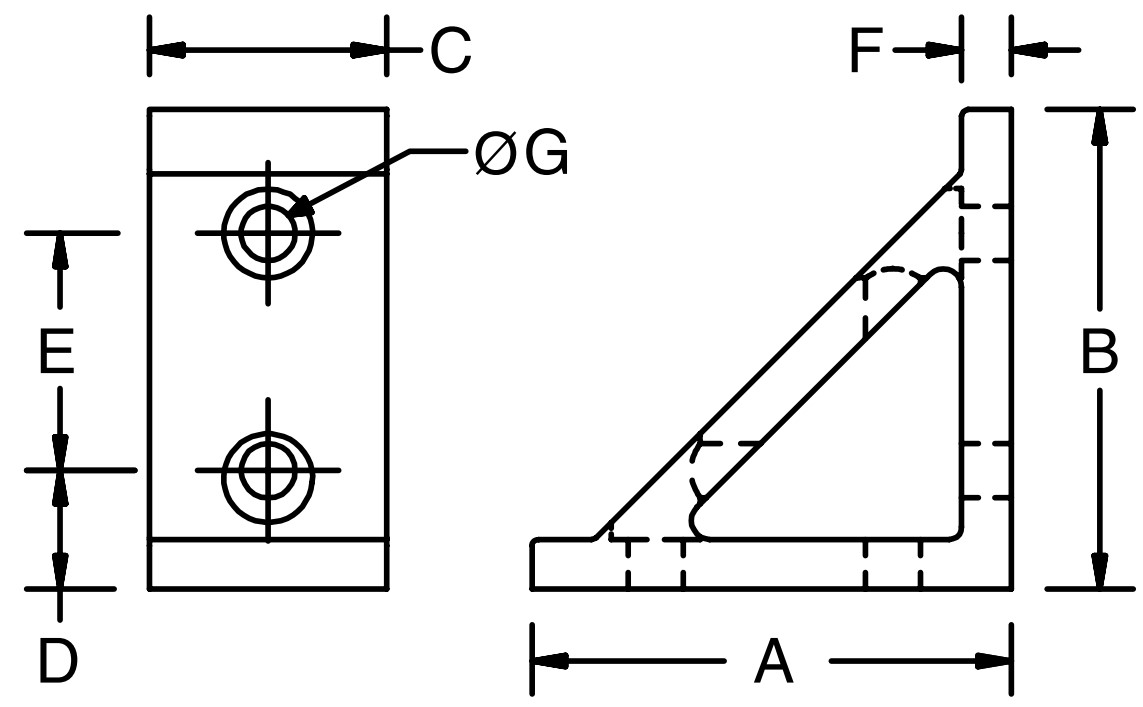
\includegraphics[width=5cm]{gusset.jpg}
	\caption{machined gusset, code \texttt{10-102}, from the IPS catalogue \cite{parker-ds}. In the drawing: $A = 77mm$, $B=77mm$, $C = 34mm$, $D= 20mm$, $E=40mm$, $F=8mm$, $G=9mm$.}
	\label{fig:gusset}
\end{SCfigure}

\paragraph{Threaded joints along the $x$ axis} The sliding actions are given by the torque $M_{zA}$, which produces a shear force on every screw equal to:\\
\begin{equation*}
    V_{i} = \frac{M_{z1}r_{i}}{\sum\limits_{i=1}^{n_{{b}}} r^2_{i}}
\end{equation*}
where $r_{i}$ are the distances of every screw from the center of the section O, and are equal to $r_{1} = 40 mm$, $r_{2} = 80 mm$. 
The shear force is calculated for the most critical screws, distant $r_{2}$ from O, and it is equal to:\\
\begin{equation*}
    V_{2} = \frac{M_{zA}r_{2}}{2r^2_{1}+2r^2_{2}} = -0.003 N
\end{equation*}
The shear and punching resistance verifications can be performed as follow:
\begin{itemize}
    \item shear resistance verification:
    \begin{equation*}
        |V_{2}| < \frac{\sigma_{uts}A_{b}}{\phi}
    \end{equation*}
    where $\sigma_{uts}$ corresponds to the screw's ultimate tensile strength, $A_{b}$ to the bolt cross-section and $\phi$ is the safety factor which, according to Eurocode3, is equal to $\frac{1.25}{0.58}$.
    As a consequence, it follows that:
    \begin{equation*}
       \sigma_{uts} > \frac{|V_{2}|\phi}{A_{b}} = 0.127 \cdot 10^{-3} MPa.
    \end{equation*}\\
    \item crushing resistance verification:
    \begin{equation*}
        |V_{2}| < \frac{\sigma_{uts,m}dt}{\phi}
    \end{equation*}
    where $\sigma_{uts,m}$ corresponds to the member's ultimate tensile strength, $d$ to the bolt diameter and $\phi$ is the safety factor which, according to Eurocode3, is equal to 0.5. Finally, $t$ corresponds to the member's thickness, which can be calculated as the sum of the machined gussets thickness, $F = 8 mm$, and the member's cross section, equal to $40 mm$.
     \begin{equation*}
       \sigma_{uts,m} > \frac{|V_{2}|\phi}{dt} = 3.314 \cdot 10^{-6} MPa.
    \end{equation*}
\end{itemize}

Separating actions are given by the axial load and the bending moments.\\
Assuming that the members are rigid it is possible to calculate the effects of the separating actions in both $xz$ and $yz$ planes.\\
The load caused by the separating action, acting on each bolt can be calculated as:\\
\begin{equation*}
    N_{i} = \frac{M_{b}h_{i}}{\sum\limits_{i=1}^{n_{b}} h^2_{i}} + \frac{N}{n_{b}}
\end{equation*}
Considering the $xz$ plane and assuming the pivot is placed on the edge of the section, the constant h$_{i}$ will be equal to:
\begin{equation*}
   \begin{cases}
    h_{1} = 16.962 mm\\
    h_{2} = 56.962 mm\\
    h_{3} = 136.962 mm\\
    h_{4} = 176.962 mm\\
    \end{cases} 
\end{equation*}
The normal load is calculated for the most critical screw as follow:\\
\begin{equation*}
    N_{xz} = \frac{M_{yA}h_{4}}{h_{1}^{2}+h_{2}^{2}+h_{3}^{2}+h_{4}^{2}} + \frac{N_{1}}{n_{b}} = -62.775 N
\end{equation*}
Since the axial load acting on every bolt is negative, i.e. the bolt are subjected to compression, there are no issues relative to tension and punching resistance. As a consequence, it is not necessary to perform those verifications. \textbf{(???)}

Considering the $yz$ plane and assuming that the pivot is placed on the edge of the section, the constants $h_{i}$ will be all equal to $\frac{C}{2} = 17 mm$.
The normal load is equal to:
\begin{equation*}
    N_{yz} = \frac{M_{xA}h_{4}}{h_{1}^{2}+h_{2}^{2}+h_{3}^{2}+h_{4}^{2}} + \frac{N_{1}}{n_{b}} = -62.596 N
\end{equation*}
Even in this case the axial load in of compression and the verifications do not have to be performed. 

\paragraph{Threaded joints along the $z$ axis} Similarly to the x axis, the axial loads are of compression. The calculations are not reported for the purpose of brevity.

\subsubsection*{Section D}
The loads applied on section $D$ are the following:
\begin{itemize}
	\item axial load $N_{D} = 233.010 N$;
	\item bending moment $M_{xD} = 0 N\cdot m$; 
	\item bending moment $M_{yD} = 8.106 N\cdot m$; 
	\item torque $M_{zD}x = -0.594 N\cdot m$.
\end{itemize}
In correspondence of section $D$, there is a pivot joint chosen from the Parker IPS catalogue \cite{parker-ds}, reported in figure \ref{fig:pivot}.
\begin{figure}[bt]
    \centering
    \begin{subfigure}{0.32\linewidth}
    	\centering 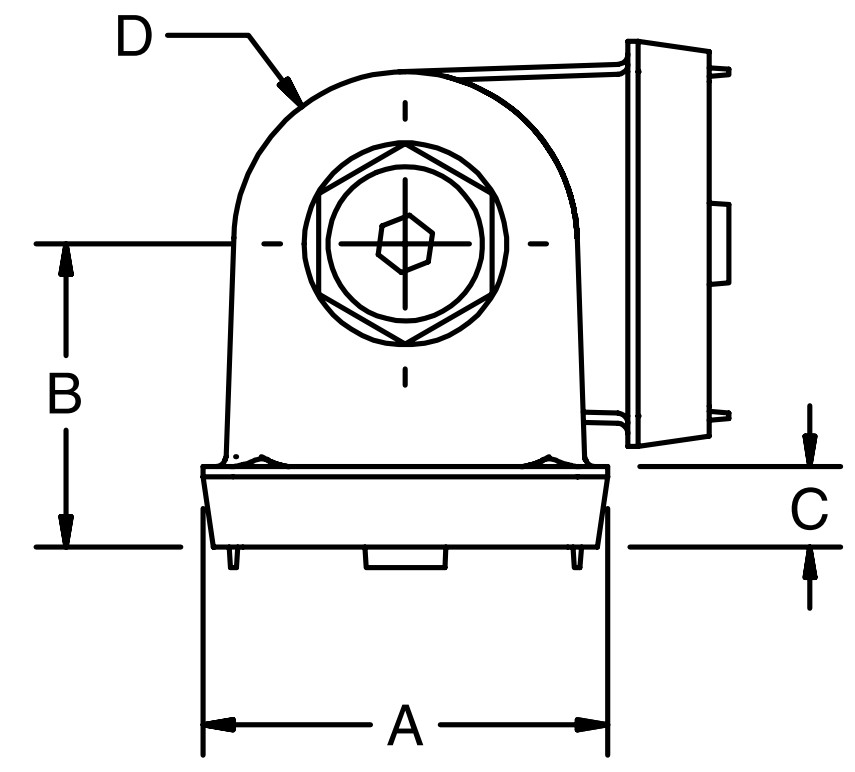
\includegraphics[width=4cm]{pivotjoint.jpg} \caption{}
    \end{subfigure}
	\begin{subfigure}{0.32\linewidth}
		\centering 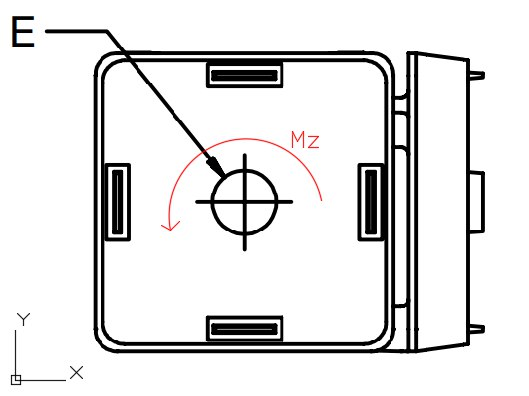
\includegraphics[width=4cm]{sectionD} \caption{}
	\end{subfigure}
	\begin{subfigure}{0.32\linewidth}
		\centering 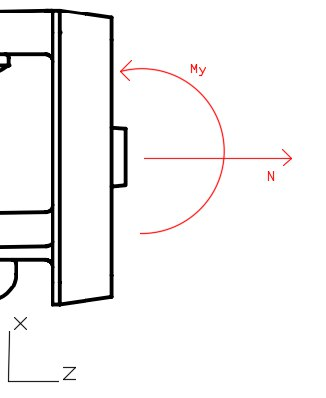
\includegraphics[width=3cm]{xz.png} \caption{}
	\end{subfigure}    
    \caption{pivot joint, code \texttt{23-010}, from the IPS catalogue \cite{parker-ds}. In the drawing: $A = 40mm$, $B=30mm$, $C=9mm$, $D=40mm$, $E=8.5mm$, $F=60mm$.}
    \label{fig:pivot}
\end{figure}

In this case, the sliding actions are given by the torque $M_{zD}$,  figure \ref{fig:pivot}\textit{(b)}. However, since there is a single screw positioned in the center of the section, they do not cause any shear on the screw. \textbf{(??)}

Separating actions are given by the axial load and the bending moments. Assuming that the members are rigid it is possible to calculate the effects of the separating actions in both $xz$ and $yz$ planes. The load caused by the separating action, acting on the screw can be calculated as:
\begin{equation*}
    N_{i} = \frac{M_{b}h_{i}}{\sum\limits_{i=1}^{n_{b}} h^2_{i}} + \frac{N}{n_{b}}
\end{equation*}\\
where $h_{i}$ is the distance of the $i$-th bolt from the pivot point.
\begin{equation*}
    N_{xz} = \frac{M_{yD}}{h} + N_{D} = 233.415 N
\end{equation*}

Considering the $xz$ plane and assuming the pivot on the edge of the section, $h$ is equal to $\frac{A}{2} = 20 mm$. The tension resistance and punching verification can be performed as follow:
\begin{itemize}
    \item tension resistance verification:
    \begin{equation*}
        N_{xz} < \frac{\sigma_{uts}A_{bt}}{\phi}
    \end{equation*}
    Where $\sigma_{uts}$ corresponds to the screw's ultimate tensile strength, $A_{bt}$ to the bolt tensile cross-section and $\phi$ is the safety factor which, according to Eurocode3, is equal to $\frac{1.25}{0.9}$. As a consequence, it follows that:
    \begin{equation*}
       \sigma_{uts} > \frac{N_{xz}\phi}{A_{bt}} = 8.858 MPa.
    \end{equation*}
    \item punching resistance verification:
    \begin{equation*}
        N_{xz} < \frac{\pi d_{0} t \sigma_{uts,m}}{\phi}
    \end{equation*}
    Where $\sigma_{uts,m}$ corresponds to the member's ultimate tensile strength, $d_{0}$ the bolt head diameter and $\phi$ is the safety factor which, according to Eurocode3, is equal to $\frac{1.25}{0.6}$. Finally, $t$ corresponds to the member's thickness, which can be calculated as the sum of the pivot joint thickness, $C = 9 mm$, and the member's cross section, equal to $40 mm$:
     \begin{equation*}
       \sigma_{uts,m} > \frac{N_{xz}\phi}{\pi d_{0}t} = 0.226 MPa.
    \end{equation*}
\end{itemize}
%\begin{figure}[h!]
%    \centering
%    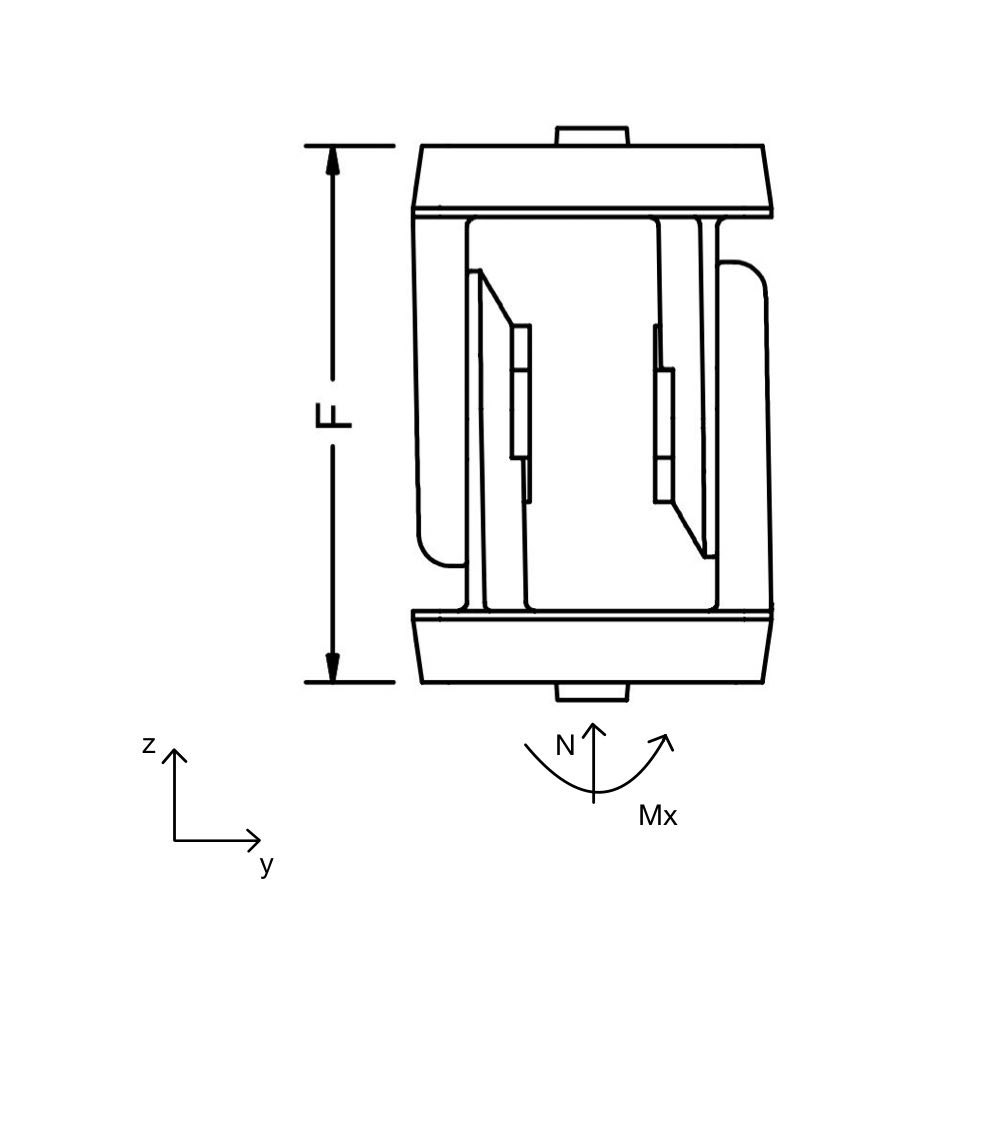
\includegraphics[width=5cm]{yz.png}
%    \caption{}
%    \label{fig:yz}
%\end{figure}
Considering instead the $xz$ plane we have:\\
\begin{equation*}
    N_{yz} = \frac{M_{xD}}{h} + N_{D} = 233.010 N
\end{equation*}
thus:
\begin{itemize}
    \item tension resistance verification:
    \begin{equation*}
        N_{yz} < \frac{\sigma_{uts}A_{bt}}{\phi} \qquad \Rightarrow \sigma_{uts} > \frac{N_{yz}\phi}{A_{bt}} = 8.842 MPa.
    \end{equation*}
    \item punching resistance verification\\
    \begin{equation*}
        N_{yz} < \frac{\pi d_{0} t \sigma_{uts,m}}{\phi} \qquad \Rightarrow \qquad   \sigma_{uts,m} > \frac{N_{yz}\phi}{\pi d_{0}t} = 0.246 MPa.
    \end{equation*}
\end{itemize}
In conclusion, the bolt ultimate strength must be greater than $8.858 MPa$, a value that allows to choose any bolt property class. In order to minimize the costs, property 4.6 is chosen.\textbf{(????)} 

Moreover, the verifications for crushing and punching provide the minimum member ultimate strength, $\sigma_{uts,m} > 0.226 MPa$, value much smaller than the chosen member's UTS.

Note that for the verifications of the separating actions the rigid member approach was used, which is usually more conservative than the others. However, since the values obtained are far distant from the one of the selected materials, there is no need of a more precise verification.
	\subsection{Static verification rack and gear}
The verification continued with the parts responsible for actuating the machine, rack that is positioned on both tracks and gear attached on the motors' shaft.
We focused on two important aspects, interference and tooth root bending resistance.

\subsubsection*{Interference condition}
It's fundamental to check if this condition is fulfilled, because otherwise we could have a problem of undercut, when the tip of the rack cutter is moved beyond the base circle of the gear and the result is the weakening of the gear's teeth.

Interference condition is function of the minimum number of teeth of the pinion, in accordance with the following equation:
\begin{equation}
	\centering
	z_{min} = \frac{2}{sin^2\alpha},
\end{equation}
where $\alpha$ is the pressure angle, as we can see in figure \ref{fig:rack}.
\begin{SCfigure}[1][hbt]
	\centering
	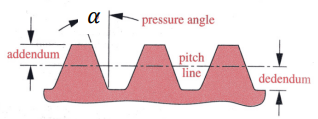
\includegraphics[scale=1]{Images/rack.png}
	\caption{standard rack and pressure angle $\alpha$.}
	\label{fig:rack}
\end{SCfigure}
In our case we designed the profile with a pressure $\alpha = 20^\circ$, thus we have:
\begin{equation*}
	z_{min} = 17,
\end{equation*}
that means that the interfence condition, in our project, is fulfilled because we designed a pinion with $z=18$.

\subsubsection*{Tooth root fatigue resistance}
One of the most important problem in the usage of gears is the teeth fatigue resistance, due to the fact they're subjected to pulsating loads.

In our analysis we used the Lewis method that consider the tooth as a cantilever beam and shear and compressive normal stresses are neglected.
In order to compute the stress state we used the following equation:
\begin{equation}
	\centering
	\sigma_L=\frac{6F_th}{bs_L^2},
	\label{stress}
\end{equation}
where $F_t$, $h$, $b$ and $s_L$ are showed in figure \ref{fig:tooth}.
\begin{figure}[bt]
\begin{subfigure}{.5\textwidth}
	\centering
	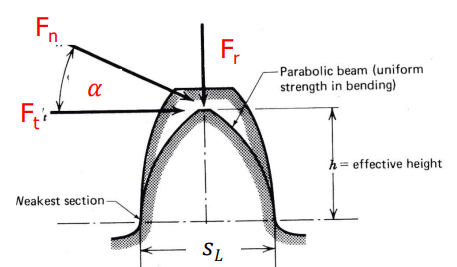
\includegraphics[scale=0.5]{Images/toothgear1.png}
	\caption{}
\end{subfigure}%
\begin{subfigure}{.5\textwidth}
	\centering
	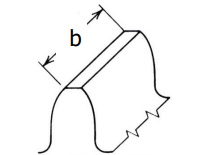
\includegraphics[scale=0.6]{Images/toothgear2.png}
	\caption{}
\end{subfigure}
\caption{tooth details: section (a) and face width (b).}
\label{fig:tooth}
\end{figure}
For our project we considered that actuation is performed by means of two motors with a nominal power $P=10W$ rotating at $\omega=50rpm$ that are attached at the prismatic joints at both ends $A$ and $D$; given the maximum torque expressed by the motor as
\begin{equation*}
	T = \frac{P}{\omega} = 1.9 N\cdot m 
\end{equation*}
the actual force $F_t$ exerted on the teeth depends on the radius $r = 17.14mm$ of the gear as
\begin{equation*}
	\centering
	F_t = \frac{T}{r} = 111.3 N
\end{equation*}
At this point we can find the stress state, from \eqref{stress}:
\begin{equation}
	\centering
	\sigma_L=\frac{6\cdot 111.3\cdot 2.14}{10\cdot 1.79^2} = 44.6 MPa
	\label{stressdata}
\end{equation}\\
The Lewis method provide the nominal stress state at the base of the tooth, in the hypothesis of considering the tooth as a cantilever beam.\\
All factors affecting the actual value of the stress state should therefore be taken into account in the design. Moreover, the admissible stress must be defined starting from the properties of the material and the production and processing techniques adopted.\\

